% ==============================================================================
% SECCIÓN 7: ARQUITECTURA DE SOFTWARE, CLEAN ARCHITECTURE, CQRS Y BASE DE DATOS
% ==============================================================================

\section{Arquitectura de Software y Diseño del Sistema}

El sistema web \textbf{SYSELL} adopta una arquitectura desacoplada y orientada al dominio, diseñada bajo los principios de \textbf{Clean Architecture} formulados por Robert C. Martin, combinados con la segregación de responsabilidades de comandos y consultas (\textbf{CQRS}). Esta estructura garantiza independencia del framework, testeabilidad exhaustiva, alta escalabilidad y facilidad de mantenimiento a largo plazo.

\subsection{Arquitectura General del Sistema (Modelo C4 --- Contenedores)}

El sistema opera bajo un esquema cliente-servidor distribuido vía API RESTful sobre HTTPS, como se ilustra en el siguiente diagrama de contenedores:

\begin{figure}[H]
\centering
\begin{tikzpicture}[
    scale=0.82, transform shape,
    node distance=1.2cm and 1.4cm,
    box/.style={rectangle, draw=PrimaryBlue, fill=LightSlate, rounded corners=3pt, text width=2.9cm, minimum height=1.4cm, align=center, font=\small},
    api/.style={rectangle, draw=SecondaryBlue, fill=white, rounded corners=3pt, text width=3.2cm, minimum height=1.6cm, align=center, font=\small},
    db/.style={cylinder, shape border rotate=90, draw=AccentTeal, fill=white, aspect=0.25, minimum width=2.6cm, minimum height=1.4cm, align=center, font=\small},
    arrow/.style={-Latex, thick, color=PrimaryBlue}
]
    % Clientes
    \node[box] (desktop) {\textbf{Cliente Web Desktop}\\ \scriptsize React 18 + TS + Vite\\ (Navegador Chrome/Edge)};
    \node[box, below=0.6cm of desktop] (mobile) {\textbf{Cliente Web Responsive}\\ \scriptsize Vista Móvil 360px\\ (Smartphones / Tablets)};

    % Proxy / Gateway
    \node[api, right=1.6cm of $(desktop)!0.5!(mobile)$] (nginx) {\textbf{Proxy Inverso Nginx}\\ \scriptsize Nginx 1.24 (Docker)\\ \scriptsize SSL/TLS 1.3 + Gzip};

    % Backend API
    \node[api, right=1.6cm of nginx] (backend) {\textbf{Backend API REST}\\ \scriptsize Laravel 11 / PHP 8.2\\ \scriptsize Clean Arch + CQRS\\ \scriptsize Sanctum Auth};

    % Base de Datos
    \node[db, right=1.6cm of backend] (mysql) {\textbf{MySQL 8.0}\\ \scriptsize Motor InnoDB\\ \scriptsize Transacciones ACID\\ \scriptsize Soft Deletes};

    % Conexiones
    \draw[arrow] (desktop.east) -- node[above, font=\tiny]{HTTPS / JSON} (nginx.west);
    \draw[arrow] (mobile.east) -- node[below, font=\tiny]{HTTPS / JSON} (nginx.west);
    \draw[arrow] (nginx.east) -- node[above, font=\tiny]{FastCGI:9000} (backend.west);
    \draw[arrow] (backend.east) -- node[above, font=\tiny]{TCP:3306} (mysql.west);
\end{tikzpicture}
\caption{Diagrama de Contenedores C4 del Sistema Web SYSELL.}
\label{fig:c4_containers}
\end{figure}

\subsection{Estructura de Capas en Clean Architecture}

La arquitectura del backend se organiza en cuatro capas concéntricas con una regla de dependencia estricta dirigida hacia el centro (\textit{Dependency Inversion Principle}):

\begin{figure}[H]
\centering
\begin{tikzpicture}[scale=0.88, every node/.style={scale=0.88}]
    % Capa Externa: Frameworks & Drivers (Radio = 5.6cm)
    \draw[fill=PrimaryBlue!12, draw=PrimaryBlue, thick] (0,0) circle (5.6cm);
    \node[text width=9.6cm, align=center] at (0, 4.8) {
        \textbf{\color{PrimaryBlue}\small Capa 4: Frameworks, Drivers \& UI}\\[0.05cm]
        \scriptsize\color{DarkSlate} Laravel Routing, MySQL 8, Nginx Web Server, React SPA, Docker
    };

    % Capa 3: Adaptadores de Interfaz / Presentación (Radio = 4.1cm)
    \draw[fill=SecondaryBlue!18, draw=SecondaryBlue, thick] (0,0) circle (4.1cm);
    \node[text width=7.6cm, align=center] at (0, 3.3) {
        \textbf{\color{SecondaryBlue}\small Capa 3: Adaptadores de Interfaz}\\[0.05cm]
        \scriptsize\color{DarkSlate} Controllers, Presenters, Eloquent Repositories, FormRequests
    };

    % Capa 2: Casos de Uso (Aplicación) (Radio = 2.6cm)
    \draw[fill=AccentTeal!22, draw=AccentTeal, thick] (0,0) circle (2.6cm);
    \node[text width=5.2cm, align=center] at (0, 1.85) {
        \textbf{\color{AccentTeal!90!black}\small Capa 2: Casos de Uso / Aplicación}\\[0.05cm]
        \scriptsize\color{DarkSlate} Command/Query Handlers, DTOs, Policies
    };

    % Capa 1: Dominio (Entidades y Reglas de Empresa) (Radio = 1.25cm)
    \draw[fill=white, draw=AlertRed, thick] (0,0) circle (1.25cm);
    \node[text width=2.4cm, align=center] at (0, 0) {
        \textbf{\color{AlertRed}\small Capa 1: Dominio}\\[0.05cm]
        \tiny\color{DarkSlate} Entidades, Value Objects, Reglas de Negocio (RN)
    };

    % Flechas de Dependencia hacia adentro
    \draw[-{Latex[scale=1.1]}, thick, color=AlertRed] (4.8, -1.8) -- node[right, font=\tiny\bfseries, color=AlertRed]{Regla de Dependencia} (2.8, -1.0);
    \draw[-{Latex[scale=1.1]}, thick, color=AlertRed] (-4.8, -1.8) -- node[left, font=\tiny\bfseries, color=AlertRed]{Hacia el Dominio} (-2.8, -1.0);
\end{tikzpicture}
\caption{Capas Concéntricas y Flujo de Dependencias en Clean Architecture.}
\label{fig:clean_arch}
\end{figure}

\begin{enumerate}[leftmargin=*]
    \item \textbf{Capa de Dominio (\textit{Core Domain}):} Contiene las entidades de negocio puras (\texttt{Sale}, \texttt{ProductVariant}, \texttt{CashRegister}, \texttt{Return}), objetos de valor (\textit{Value Objects}) y las reglas de negocio independientes de cualquier base de datos o framework.
    \item \textbf{Capa de Aplicación (\textit{Application / Use Cases}):} Orquesta el flujo de datos y la ejecución de los casos de uso a través del patrón CQRS. Define interfaces de repositorios (\texttt{SaleRepositoryInterface}) e interactúa mediante objetos de transferencia (\textit{DTOs}).
    \item \textbf{Capa de Adaptadores de Interfaz (\textit{Interface Adapters}):} Traduce los datos entre los casos de uso y los agentes externos. Incluye los controladores de la API REST (\texttt{SaleApiController}), los \textit{FormRequests} de validación, los \textit{Transformers/Resources} de salida JSON y las implementaciones concretas de repositorios con Eloquent ORM.
    \item \textbf{Capa de Infraestructura (\textit{Frameworks \& Drivers}):} Aloja los detalles técnicos: conexión con el motor MySQL 8, motor de correo SMTP, servicios de generación de PDFs (\texttt{DomPDF}), middleware de autenticación (Sanctum) y servicios del sistema operativo.
\end{enumerate}

\subsection{Implementación del Patrón CQRS (Command Query Responsibility Segregation)}

Para maximizar el rendimiento y la consistencia transaccional, las operaciones sobre el sistema se bifurcan en dos flujos especializados:

\begin{figure}[H]
\centering
\begin{tikzpicture}[
    scale=0.88, transform shape,
    node distance=1.2cm and 1.4cm,
    comp/.style={rectangle, draw=DarkSlate, fill=white, rounded corners=3pt, text width=2.8cm, minimum height=1.2cm, align=center, font=\small},
    cmd/.style={rectangle, draw=AlertRed, fill=AlertRed!10, rounded corners=3pt, text width=2.8cm, minimum height=1.2cm, align=center, font=\small},
    qry/.style={rectangle, draw=SuccessGreen, fill=SuccessGreen!10, rounded corners=3pt, text width=2.8cm, minimum height=1.2cm, align=center, font=\small},
    db/.style={cylinder, shape border rotate=90, draw=PrimaryBlue, fill=LightSlate, aspect=0.25, minimum width=2.4cm, minimum height=1.4cm, align=center, font=\small},
    arrow/.style={-Latex, thick}
]
    % Cliente / API
    \node[comp] (controller) {\textbf{API REST Controller}\\ \scriptsize Recibe HTTP POST/GET};

    % Flujo de Comandos (Mutaciones)
    \node[cmd, above right=0.6cm and 1.2cm of controller] (cmdBus) {\textbf{Command Handler}\\ \scriptsize \texttt{CreateSaleCommand}\\ \scriptsize Dominio \& RN};
    \node[cmd, right=1.0cm of cmdBus] (writeRepo) {\textbf{Write Repository}\\ \scriptsize Eloquent ORM\\ \scriptsize Transacción ACID};

    % Flujo de Consultas (Lecturas)
    \node[qry, below right=0.6cm and 1.2cm of controller] (qryBus) {\textbf{Query Handler}\\ \scriptsize \texttt{GetSalesReportQuery}\\ \scriptsize Filtros optimizados};
    \node[qry, right=1.0cm of qryBus] (readModel) {\textbf{Read Model / DTO}\\ \scriptsize Vistas / Índices MySQL\\ \scriptsize Respuestas JSON};

    % Base de Datos
    \node[db, right=1.2cm of $(writeRepo)!0.5!(readModel)$] (mysql) {\textbf{MySQL 8.0}\\ \scriptsize Esquema Relacional};

    % Conexiones
    \draw[arrow, color=AlertRed] (controller.north) |- node[above, font=\tiny]{Comando (POST/PUT/DELETE)} (cmdBus.west);
    \draw[arrow, color=AlertRed] (cmdBus.east) -- (writeRepo.west);
    \draw[arrow, color=AlertRed] (writeRepo.east) -| (mysql.north);

    \draw[arrow, color=SuccessGreen] (controller.south) |- node[below, font=\tiny]{Consulta (GET)} (qryBus.west);
    \draw[arrow, color=SuccessGreen] (qryBus.east) -- (readModel.west);
    \draw[arrow, color=SuccessGreen] (mysql.south) |- (readModel.east);
\end{tikzpicture}
\caption{Flujo de Ejecución de Comandos y Consultas (CQRS) en SYSELL.}
\label{fig:cqrs_flow}
\end{figure}

\subsection{Modelo de Datos Relacional y Esquema de Base de Datos}

El diseño de la base de datos en \textbf{MySQL 8.0} está normalizado en Tercera Forma Normal (3FN) e incorpora columnas obligatorias de auditoría (\texttt{created\_at}, \texttt{updated\_at}, \texttt{deleted\_at}) para todas las tablas principales:

\begin{figure}[H]
\centering
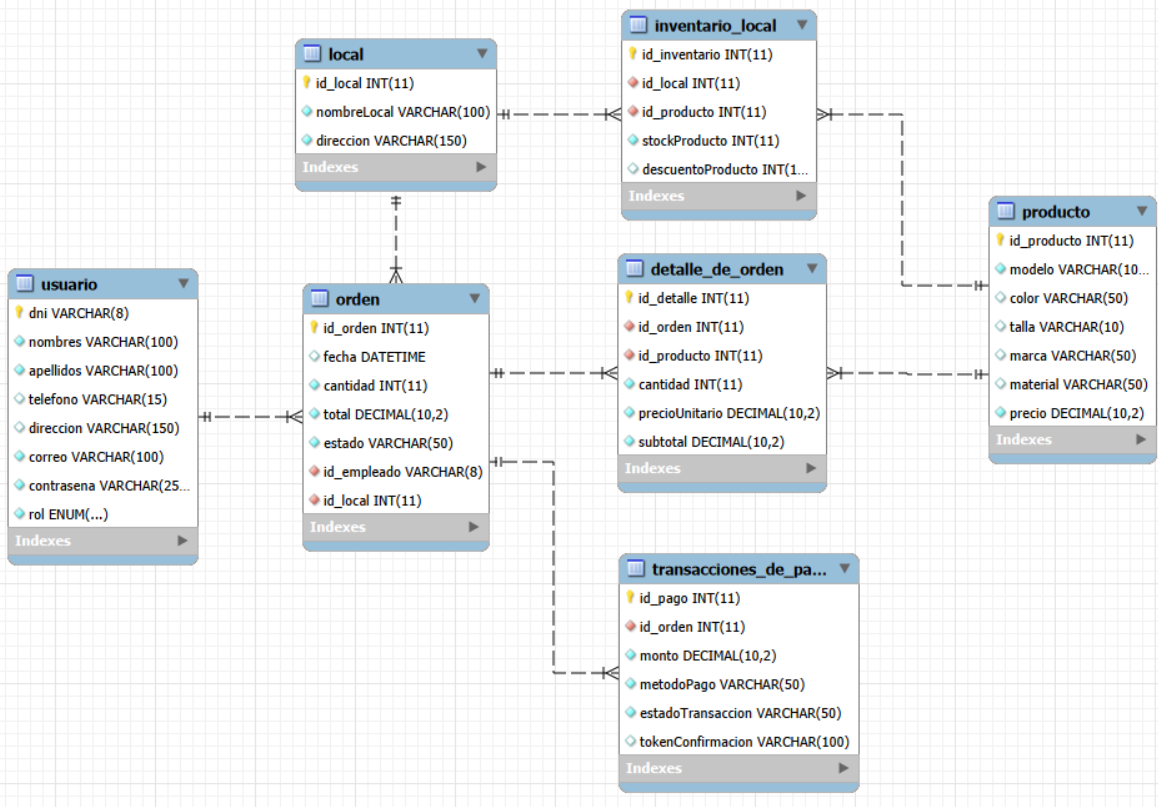
\includegraphics[width=0.92\linewidth]{figures/diagrama_bd_original.png}
\caption{Diagrama de Base de Datos y Entidades Relacionales de SYSELL.}
\label{fig:diagrama_bd}
\end{figure}

\begin{table}[H]
\centering
\small
\begin{tabularx}{\linewidth}{l>{\raggedright\arraybackslash}p{4cm}>{\raggedright\arraybackslash}X}
\toprule
\rowcolor{LightSlate}
\textbf{Tabla} & \textbf{Clave Primaria / Foráneas} & \textbf{Descripción y Campos Principales} \\
\midrule
\texttt{users} & \texttt{id} (PK), \texttt{store\_id} (FK) & Usuarios y empleados: \texttt{name}, \texttt{dni}, \texttt{phone}, \texttt{email}, \texttt{password\_hash}, \texttt{role} (\texttt{admin}/\texttt{seller}), \texttt{deleted\_at}. \\
\midrule
\texttt{stores} & \texttt{id} (PK) & Locales y almacenes: \texttt{name}, \texttt{address}, \texttt{phone}, \texttt{is\_active}, \texttt{deleted\_at}. \\
\midrule
\texttt{categories} & \texttt{id} (PK), \texttt{parent\_id} (FK) & Categorías jerárquicas: \texttt{name}, \texttt{slug}, \texttt{description}, \texttt{deleted\_at}. \\
\midrule
\texttt{products} & \texttt{id} (PK), \texttt{category\_id} (FK) & Productos padre: \texttt{name}, \texttt{brand}, \texttt{season}, \texttt{base\_price}, \texttt{base\_cost}, \texttt{image\_url}, \texttt{deleted\_at}. \\
\midrule
\texttt{product\_variants} & \texttt{id} (PK), \texttt{product\_id} (FK), \texttt{store\_id} (FK) & Variantes físicas: \texttt{sku}, \texttt{size}, \texttt{color}, \texttt{stock\_current}, \texttt{stock\_minimo}, \texttt{price\_override}. \\
\midrule
\texttt{sales} & \texttt{id} (PK), \texttt{user\_id} (FK), \texttt{store\_id} (FK), \texttt{cash\_register\_id} (FK) & Cabecera de venta: \texttt{sale\_number}, \texttt{subtotal}, \texttt{tax\_igv} (18\%), \texttt{total}, \texttt{payment\_method} (\texttt{cash}/\texttt{yape\_plin}/\texttt{transfer}), \texttt{operation\_code}, \texttt{status}, \texttt{deleted\_at}. \\
\midrule
\texttt{sale\_items} & \texttt{id} (PK), \texttt{sale\_id} (FK), \texttt{variant\_id} (FK) & Detalle de venta: \texttt{quantity}, \texttt{unit\_price}, \texttt{unit\_cost}, \texttt{subtotal}. \\
\midrule
\texttt{cash\_registers} & \texttt{id} (PK), \texttt{store\_id} (FK), \texttt{user\_id} (FK) & Sesiones de caja: \texttt{opening\_amount}, \texttt{closing\_cash\_counted}, \texttt{closing\_digital\_counted}, \texttt{expected\_amount}, \texttt{difference}, \texttt{status} (\texttt{open}/\texttt{closed}), \texttt{opened\_at}, \texttt{closed\_at}. \\
\midrule
\texttt{returns} & \texttt{id} (PK), \texttt{sale\_id} (FK), \texttt{user\_id} (FK) & Devoluciones y cambios: \texttt{returned\_variant\_id}, \texttt{new\_variant\_id}, \texttt{difference\_amount}, \texttt{reason}, \texttt{returned\_at}. \\
\midrule
\texttt{audit\_logs} & \texttt{id} (PK), \texttt{user\_id} (FK) & Bitácora de auditoría: \texttt{action}, \texttt{entity\_type}, \texttt{entity\_id}, \texttt{old\_values\_json}, \texttt{new\_values\_json}, \texttt{ip\_address}, \texttt{created\_at}. \\
\bottomrule
\end{tabularx}
\caption{Diccionario del Esquema Relacional de Base de Datos.}
\label{tab:diccionario_bd}
\end{table}

\subsection{Diagrama de Clases del Dominio}

\begin{figure}[H]
\centering
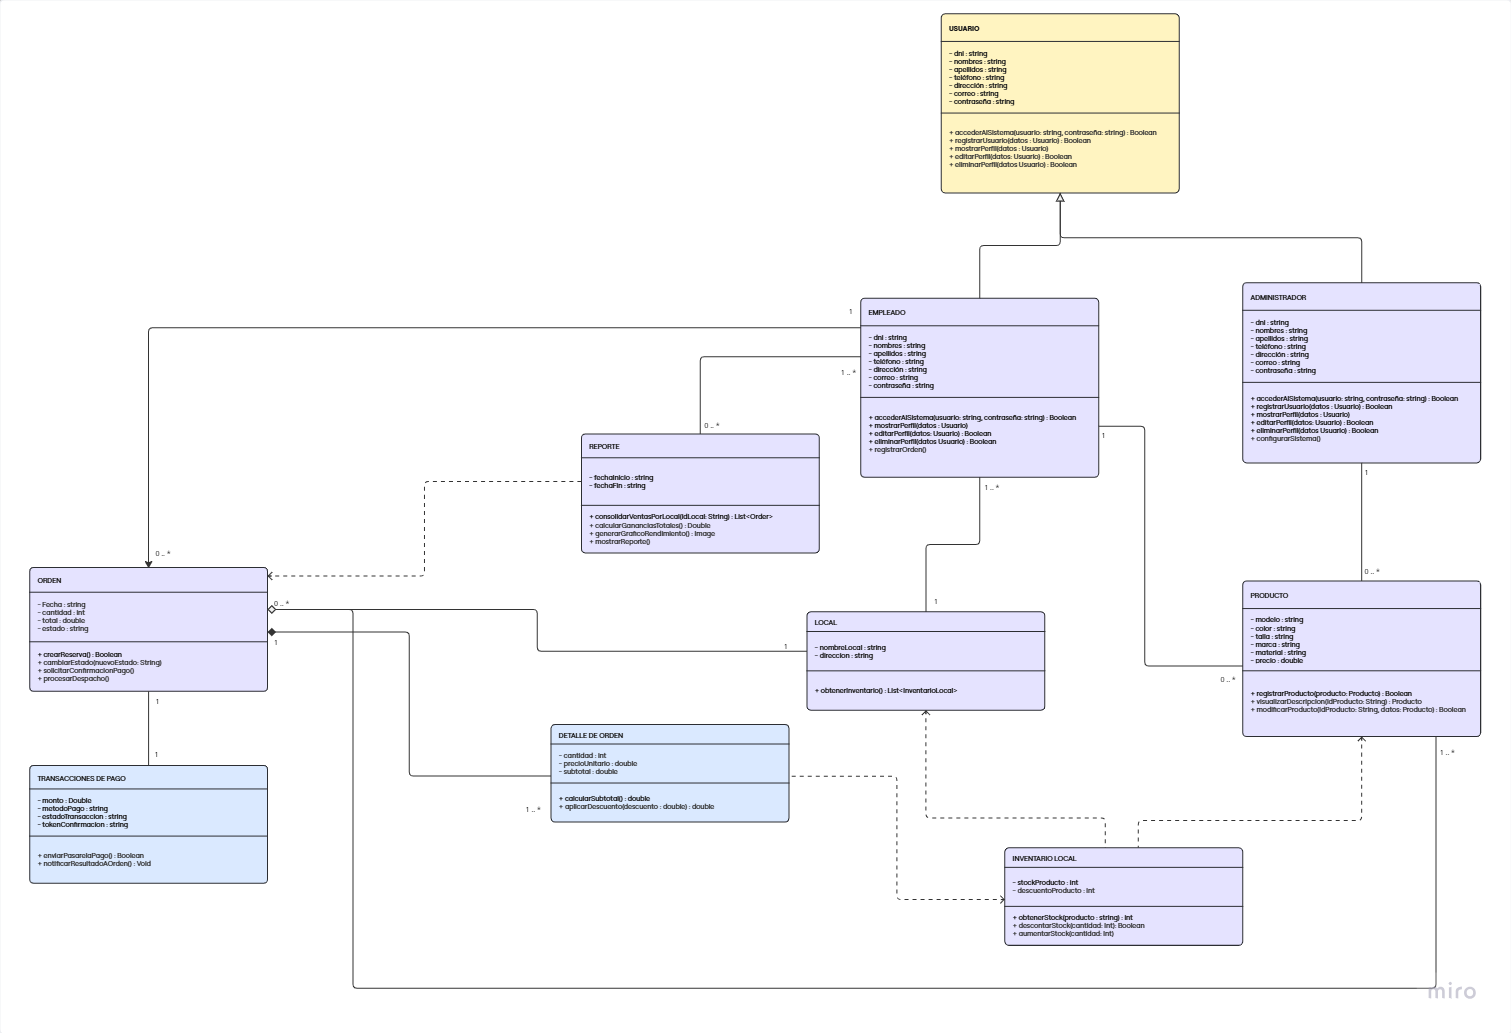
\includegraphics[width=0.88\linewidth]{figures/diagrama_clases_completo.png}
\caption{Diagrama de Clases y Relaciones de Dominio en SYSELL.}
\label{fig:diagrama_clases}
\end{figure}

\subsection{Entorno de Contenerización y DevOps (Docker \& CI/CD)}

El despliegue del sistema se encuentra completamente automatizado mediante Docker Compose:

\begin{lstlisting}[language=SQL, caption={Configuración de Servicios en \texttt{docker-compose.yml} (Extracto Estructurado)}]
version: '3.8'
services:
  sysell-frontend:
    build:
      context: ./frontend
      dockerfile: Dockerfile
    ports:
      - "80:80"
    depends_on:
      - sysell-backend

  sysell-backend:
    build:
      context: ./backend
      dockerfile: Dockerfile
    environment:
      APP_ENV: production
      DB_CONNECTION: mysql
      DB_HOST: sysell-db
      DB_DATABASE: sysell_db
      DB_USERNAME: sysell_user
      DB_PASSWORD: ${DB_PASSWORD}
    depends_on:
      - sysell-db

  sysell-db:
    image: mysql:8.0
    command: --default-authentication-plugin=mysql_native_password
    volumes:
      - mysql_data:/var/lib/mysql
    environment:
      MYSQL_DATABASE: sysell_db
      MYSQL_ROOT_PASSWORD: ${MYSQL_ROOT_PASSWORD}

volumes:
  mysql_data:
\end{lstlisting}
